Tienes un gráfico dirigido $G$ con vértices $V$ y aristas $E$. Es posible que haya bucles y múltiples aristas. Denotemos $n$ como número de vértices y $m$ como número de aristas en $G$.

Una \textbf{componente fuertemente conexa (\emph{strongly connected component,scc})} es un subconjunto máximo de vértices $C$ tal que dos vértices cualquiera de este subconjunto son accesibles entre sí, es decir, para cualquier $u, v \in C$ :

$$u \mapsto v, v \mapsto u$$

donde $\mapsto$ significa accesibilidad, es decir, existencia del camino desde el primer vértice hasta el segundo.

% TODO: \usepackage{graphicx} required
\begin{figure}[h!]
	\centering
	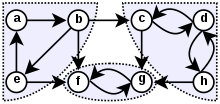
\includegraphics[width=0.4\linewidth]{img/scc}
	\label{fig:scc}
\end{figure}

En grafo se muestra arriba podemos ver que cuenta con 8 nodos y 14 aristas. Dentro del grafo se hallan tres componentes fuertemente conexa  las cuales como se observa en la figura están encerradas dentro de lineas discontinuas. De como hallarlas dado el grafo dirigido veremos en la siguiente guía. 
